%%%%%%%%%%%%%%%%%%%%%%%%%%%%%%%%%%%%%%%%%
% Classicthesis Typographic Thesis
% LaTeX Template
% Version 1.3 (15/2/14)
%
% This template has been downloaded from:
% http://www.LaTeXTemplates.com
%
% Original author:
% André Miede (http://www.miede.de)
%
% License:
% CC BY-NC-SA 3.0 (http://creativecommons.org/licenses/by-nc-sa/3.0/)
%
% General Tips:
% 1) Make sure to edit the classicthesis-config.file
% 2) New enumeration (A., B., C., etc in small caps): \begin{aenumerate} \end{aenumerate}
% 3) For margin notes: \marginpar or \graffito{}
% 4) Do not use bold fonts in this style, it is designed around them
% 5) Use tables as in the examples
% 6) See classicthesis-preamble.sty for useful commands
%
%%%%%%%%%%%%%%%%%%%%%%%%%%%%%%%%%%%%%%%%%

%----------------------------------------------------------------------------------------
%	PACKAGES AND OTHER DOCUMENT CONFIGURATIONS
%----------------------------------------------------------------------------------------

\documentclass[
		twoside,openright,titlepage,numbers=noenddot,headinclude,%1headlines,
                footinclude=true,cleardoublepage=empty,
                BCOR=5mm,paper=a4,fontsize=11pt, % Binding correction, paper type and font size
                ]{scrreprt} 
                
% Includes the file which contains all the document configurations and packages - make sure to edit this file
%%%%%%%%%%%%%%%%%%%%%%%%%%%%%%%%%%%%%%%%%
% Thesis Configuration File
%
% The main lines to change in this file are in the DOCUMENT VARIABLES
% section, the rest of the file is for advanced configuration.
%
%%%%%%%%%%%%%%%%%%%%%%%%%%%%%%%%%%%%%%%%%

%----------------------------------------------------------------------------------------
%	DOCUMENT VARIABLES
%	Fill in the lines below to enter your information into the thesis template
%	Each of the commands can be cited anywhere in the thesis
%----------------------------------------------------------------------------------------

% Remove drafting to get rid of the '[ Date - classicthesis version 4.0 ]' text at the bottom of every page
\PassOptionsToPackage{eulerchapternumbers,listings, pdfspacing, subfig,beramono,eulermath,parts, dottedtoc}{classicthesis}
% Available options: drafting parts nochapters linedheaders eulerchapternumbers beramono eulermath pdfspacing minionprospacing tocaligned dottedtoc manychapters listings floatperchapter subfig
% Adding 'dottedtoc' will make page numbers in the table of contents flushed right with dots leading to them

\newcommand{\myTitle}{Sulla correzione ortografica automatica\xspace}
\newcommand{\mySubtitle}{Un'applicazione concreta partendo da Wikipedia\xspace}
\newcommand{\myDegree}{Doktor-Ingenieur (Dr.-Ing.)\xspace}
\newcommand{\myName}{Luca Chiodini\xspace}
\newcommand{\myProf}{Put name here\xspace}
\newcommand{\myOtherProf}{Put name here\xspace}
\newcommand{\mySupervisor}{Put name here\xspace}
\newcommand{\myFaculty}{Put data here\xspace}
\newcommand{\myDepartment}{Put data here\xspace}
\newcommand{\myUni}{ITIS P. Paleocapa\xspace}
\newcommand{\myLocation}{Darmstadt\xspace}
\newcommand{\myTime}{Esame di Stato 2015\xspace}
\newcommand{\myVersion}{versione 1.0\xspace}

%----------------------------------------------------------------------------------------
%	USEFUL COMMANDS
%----------------------------------------------------------------------------------------

\newcommand{\ie}{i.\,e.}
\newcommand{\Ie}{I.\,e.}
\newcommand{\eg}{e.\,g.}
\newcommand{\Eg}{E.\,g.} 

\newcounter{dummy} % Necessary for correct hyperlinks (to index, bib, etc.)
\providecommand{\mLyX}{L\kern-.1667em\lower.25em\hbox{Y}\kern-.125emX\@}

%----------------------------------------------------------------------------------------
%	PACKAGES
%----------------------------------------------------------------------------------------

%------------------------------------------------

\usepackage{lipsum} % Used for inserting dummy 'Lorem ipsum' text into the template

%------------------------------------------------
 
%\PassOptionsToPackage{latin9}{inputenc} % latin9 (ISO-8859-9) = latin1+"Euro sign"
%\usepackage{inputenc}
\usepackage[utf8]{inputenc}


 %------------------------------------------------

%\PassOptionsToPackage{ngerman,american}{babel}  % Change this to your language(s)
% Spanish languages need extra options in order to work with this template
%\PassOptionsToPackage{spanish,es-lcroman}{babel}
%\usepackage{babel}
\usepackage[italian]{babel}

%------------------------------------------------			

\PassOptionsToPackage{square,numbers}{natbib}
 \usepackage{natbib}
 
 %------------------------------------------------

\PassOptionsToPackage{fleqn}{amsmath} % Math environments and more by the AMS 
 \usepackage{amsmath}
 % Custom
\DeclareMathOperator*{\argmax}{arg\,max}

 
 %------------------------------------------------

\PassOptionsToPackage{T1}{fontenc} % T2A for cyrillics
\usepackage{fontenc}

%------------------------------------------------

\usepackage{xspace} % To get the spacing after macros right

%------------------------------------------------

\usepackage{mparhack} % To get marginpar right

%------------------------------------------------

\usepackage{fixltx2e} % Fixes some LaTeX stuff 

%------------------------------------------------

\PassOptionsToPackage{smaller}{acronym} % Include printonlyused in the first bracket to only show acronyms used in the text
\usepackage{acronym} % nice macros for handling all acronyms in the thesis

%------------------------------------------------

%\renewcommand*{\acsfont}[1]{\textssc{#1}} % For MinionPro
\renewcommand{\bflabel}[1]{{#1}\hfill} % Fix the list of acronyms

%------------------------------------------------

\PassOptionsToPackage{pdftex}{graphicx}
\usepackage{graphicx} 


%----------------------------------------------------------------------------------------
%	FLOATS: TABLES, FIGURES AND CAPTIONS SETUP
%----------------------------------------------------------------------------------------

\usepackage{tabularx} % Better tables
\setlength{\extrarowheight}{3pt} % Increase table row height
\newcommand{\tableheadline}[1]{\multicolumn{1}{c}{\spacedlowsmallcaps{#1}}}
\newcommand{\myfloatalign}{\centering} % To be used with each float for alignment
\usepackage{caption}
\captionsetup{format=hang,font=small}
\usepackage{subfig}  

%----------------------------------------------------------------------------------------
%	CODE LISTINGS SETUP
%----------------------------------------------------------------------------------------

\usepackage{listings} 
%\lstset{emph={trueIndex,root},emphstyle=\color{BlueViolet}}%\underbar} % for special keywords
\lstset{language=[LaTeX]Tex, % Specify the language for listings here
keywordstyle=\color{RoyalBlue}, % Add \bfseries for bold
basicstyle=\small\ttfamily, % Makes listings a smaller font size and a different font
%identifierstyle=\color{NavyBlue}, % Color of text inside brackets
commentstyle=\color{Green}\ttfamily, % Color of comments
stringstyle=\rmfamily, % Font type to use for strings
numbers=left, % Change left to none to remove line numbers
numberstyle=\scriptsize, % Font size of the line numbers
stepnumber=5, % Increment of line numbers
numbersep=8pt, % Distance of line numbers from code listing
showstringspaces=false, % Sets whether spaces in strings should appear underlined
breaklines=true, % Force the code to stay in the confines of the listing box
%frameround=ftff, % Uncomment for rounded frame
frame=single, % Frame border - none/leftline/topline/bottomline/lines/single/shadowbox/L
belowcaptionskip=.75\baselineskip % Space after the "Listing #: Desciption" text and the listing box
}

%----------------------------------------------------------------------------------------
%	HYPERREFERENCES
%----------------------------------------------------------------------------------------

\PassOptionsToPackage{pdftex,hyperfootnotes=false,pdfpagelabels}{hyperref}
\usepackage{hyperref}  % backref linktocpage pagebackref
\pdfcompresslevel=9
\pdfadjustspacing=1

\hypersetup{
% Uncomment the line below to remove all links (to references, figures, tables, etc)
%draft, 
colorlinks=true, linktocpage=true, pdfstartpage=3, pdfstartview=FitV,
% Uncomment the line below if you want to have black links (e.g. for printing black and white)
%colorlinks=false, linktocpage=false, pdfborder={0 0 0}, pdfstartpage=3, pdfstartview=FitV, 
breaklinks=true, pdfpagemode=UseNone, pageanchor=true, pdfpagemode=UseOutlines,
plainpages=false, bookmarksnumbered, bookmarksopen=true, bookmarksopenlevel=1,
hypertexnames=true, pdfhighlight=/O, urlcolor=webbrown, linkcolor=RoyalBlue, citecolor=webgreen,
%------------------------------------------------
% PDF file meta-information
pdftitle={\myTitle},
pdfauthor={\textcopyright\ \myName, \myUni, \myFaculty},
pdfsubject={},
pdfkeywords={},
pdfcreator={pdfLaTeX},
pdfproducer={LaTeX with hyperref and classicthesis}
%------------------------------------------------
}   

%----------------------------------------------------------------------------------------
%	BACKREFERENCES
%----------------------------------------------------------------------------------------

\usepackage{ifthen} % Allows the user of the \ifthenelse command
\newboolean{enable-backrefs} % Variable to enable backrefs in the bibliography
\setboolean{enable-backrefs}{false} % Variable value: true or false

\newcommand{\backrefnotcitedstring}{\relax} % (Not cited.)
\newcommand{\backrefcitedsinglestring}[1]{(Cited on page~#1.)}
\newcommand{\backrefcitedmultistring}[1]{(Cited on pages~#1.)}
\ifthenelse{\boolean{enable-backrefs}} % If backrefs were enabled
{
\PassOptionsToPackage{hyperpageref}{backref}
\usepackage{backref} % to be loaded after hyperref package 
\renewcommand{\backreftwosep}{ and~} % separate 2 pages
\renewcommand{\backreflastsep}{, and~} % separate last of longer list
\renewcommand*{\backref}[1]{}  % disable standard
\renewcommand*{\backrefalt}[4]{% detailed backref
\ifcase #1 
\backrefnotcitedstring
\or
\backrefcitedsinglestring{#2}
\else
\backrefcitedmultistring{#2}
\fi}
}{\relax} 

%----------------------------------------------------------------------------------------
%	AUTOREFERENCES SETUP
%	Redefines how references in text are prefaced for different 
%	languages (e.g. "Section 1.2" or "section 1.2")
%----------------------------------------------------------------------------------------

\makeatletter
\@ifpackageloaded{babel}
{
\addto\extrasamerican{
\renewcommand*{\figureautorefname}{Figure}
\renewcommand*{\tableautorefname}{Table}
\renewcommand*{\partautorefname}{Part}
\renewcommand*{\chapterautorefname}{Chapter}
\renewcommand*{\sectionautorefname}{Section}
\renewcommand*{\subsectionautorefname}{Section}
\renewcommand*{\subsubsectionautorefname}{Section}
}
\addto\extrasngerman{
\renewcommand*{\paragraphautorefname}{Absatz}
\renewcommand*{\subparagraphautorefname}{Unterabsatz}
\renewcommand*{\footnoteautorefname}{Fu\"snote}
\renewcommand*{\FancyVerbLineautorefname}{Zeile}
\renewcommand*{\theoremautorefname}{Theorem}
\renewcommand*{\appendixautorefname}{Anhang}
\renewcommand*{\equationautorefname}{Gleichung}
\renewcommand*{\itemautorefname}{Punkt}
}
\providecommand{\subfigureautorefname}{\figureautorefname} % Fix to getting autorefs for subfigures right
}{\relax}
\makeatother

%----------------------------------------------------------------------------------------

\usepackage{classicthesis} 

%----------------------------------------------------------------------------------------
%	CHANGING TEXT AREA 
%----------------------------------------------------------------------------------------

%\linespread{1.05} % a bit more for Palatino
%\areaset[current]{312pt}{761pt} % 686 (factor 2.2) + 33 head + 42 head \the\footskip
%\setlength{\marginparwidth}{7em}%
%\setlength{\marginparsep}{2em}%

%----------------------------------------------------------------------------------------
%	USING DIFFERENT FONTS
%----------------------------------------------------------------------------------------

%\usepackage[oldstylenums]{kpfonts} % oldstyle notextcomp
%\usepackage[osf]{libertine}
%\usepackage{hfoldsty} % Computer Modern with osf
%\usepackage[light,condensed,math]{iwona}
%\renewcommand{\sfdefault}{iwona}
%\usepackage{lmodern} % <-- no osf support :-(
%\usepackage[urw-garamond]{mathdesign} <-- no osf support :-(



%------------------------------------------------
% Custom
\usepackage[binary-units=true]{siunitx}
\usepackage{tikz}
\usepackage{epigraph}
\newcommand{\shellcmd}[1]{\\\indent\indent\texttt{\footnotesize\$ #1}\\}

%\usepackage{draftwatermark}



\colorlet{punct}{red!60!black}
\definecolor{delim}{RGB}{20,105,176}
\colorlet{numb}{magenta!60!black}

\lstdefinelanguage{json}{
    basicstyle=\normalfont\ttfamily,
    numbers=left,
    numberstyle=\scriptsize,
    stepnumber=1,
    numbersep=8pt,
    showstringspaces=false,
    breaklines=true,
    frame=lines,
    literate=
     *{0}{{{\color{numb}0}}}{1}
      {1}{{{\color{numb}1}}}{1}
      {2}{{{\color{numb}2}}}{1}
      {3}{{{\color{numb}3}}}{1}
      {4}{{{\color{numb}4}}}{1}
      {5}{{{\color{numb}5}}}{1}
      {6}{{{\color{numb}6}}}{1}
      {7}{{{\color{numb}7}}}{1}
      {8}{{{\color{numb}8}}}{1}
      {9}{{{\color{numb}9}}}{1}
      {:}{{{\color{punct}{:}}}}{1}
      {,}{{{\color{punct}{,}}}}{1}
      {\{}{{{\color{delim}{\{}}}}{1}
      {\}}{{{\color{delim}{\}}}}}{1}
      {[}{{{\color{delim}{[}}}}{1}
      {]}{{{\color{delim}{]}}}}{1},
}

% No indent new paragraphs
\usepackage[parfill]{parskip}
\usepackage{mdframed}

\mdfdefinestyle{indepth}{%
  backgroundcolor=black!10!white,
  topline=false,
  rightline=false,
  leftline=false
}


\begin{document}

%\frenchspacing % Reduces space after periods to make text more compact

\raggedbottom % Makes all pages the height of the text on that page

%\selectlanguage{american} % Select your default language - e.g. american or ngerman

%\renewcommand*{\bibname}{new name} % Uncomment to change the name of the bibliography
%\setbibpreamble{} % Uncomment to include a preamble to the bibliography - some text before the reference list starts

\pagenumbering{roman} % Roman page numbering prior to the start of the thesis content (i, ii, iii, etc)

\pagestyle{plain} % Suppress headers for the pre-content pages

%----------------------------------------------------------------------------------------
%	PRE-CONTENT THESIS PAGES
%----------------------------------------------------------------------------------------

% Title Page

\begin{titlepage}

\begin{addmargin}[-1cm]{-3cm}
\begin{center}
\large

\hfill
\vfill

\begingroup
\color{Maroon}\spacedallcaps{\myTitle} \\ \bigskip % Thesis title
\endgroup

\spacedlowsmallcaps{\myName} % Your name

\vfill

%\includegraphics[width=6cm]{gfx/TFZsuperellipse_bw} \\ \medskip % Picture

\mySubtitle \\ \bigskip \bigskip % Thesis subtitle
\vfill \vfill
%\myDegree \\
%\myDepartment \\
%\myFaculty \\
\myUni \\ \medskip

%\myTime\ -- \myVersion % Time and version
\myTime

\vfill

\end{center}
\end{addmargin}

\end{titlepage} % Main title page

% Back of the title page

\thispagestyle{empty}

\hfill

\vfill

\noindent\myName: \textit{\myTitle,} \mySubtitle %\myDegree, 
%\textcopyright\ 
\\ \myTime

% You may wish to do something with the back of the title page, such as including your supervisors, location or time frame of the work. Below is an example of doing so although you may want to tweak it to your liking.

%\bigskip

%\noindent\spacedlowsmallcaps{Supervisors}: \\
%\myProf \\
%\myOtherProf \\ 
%\mySupervisor

%\medskip \\

%\noindent\spacedlowsmallcaps{Location}: \\
%\myLocation

%\medskip \\

%\noindent\spacedlowsmallcaps{Time Frame}: \\
%\myTime
 % Back of the title page

%\cleardoublepage% Dedication

\thispagestyle{empty}
\refstepcounter{dummy}

\pdfbookmark[1]{Dedication}{Dedication} % Bookmark name visible in a PDF viewer

\vspace*{3cm}

\begin{center}
\emph{Ohana} means family. \\
Family means nobody gets left behind, or forgotten. \\ \medskip
--- Lilo \& Stitch    
\end{center}

\medskip

\begin{center}
Dedicated to the loving memory of Rudolf Miede. \\ \smallskip
1939\,--\,2005
\end{center} % Dedication page

%\cleardoublepage\include{FrontBackMatter/Foreword} % Uncomment and create a Foreword.tex to include a foreword

\cleardoublepage% Abstract

\pdfbookmark[1]{Sommario}{Sommario} % Bookmark name visible in a PDF viewer

\begingroup
\let\clearpage\relax
\let\cleardoublepage\relax
\let\cleardoublepage\relax

\chapter*{Sommario} % Abstract name

Obiettivo del lavoro è costruire un sistema che proponga una correzione automatica di parole e frasi, con un approccio statistico. La sorgente dei dati su cui lavora l'algoritmo di correzione è la celebre enciclopedia Wikipedia, in lingua italiana. Si espone un servizio di API e una semplice applicazione web per gli utenti finali. Si pone particolare accento all'intera implementazione con un occhio di riguardo per l’ottimizzazione. 

\endgroup			

\vfill
 % Abstract page

%\cleardoublepage% Publications - a page listing research articles written using content in the thesis

\pdfbookmark[1]{Publications}{Publications} % Bookmark name visible in a PDF viewer

\chapter*{Publications} % Publications page text

Some ideas and figures have appeared previously in the following publications:

\bigskip

\noindent Put your publications from the thesis here. The packages \texttt{multibib} or \texttt{bibtopic} etc. can be used to handle multiple different bibliographies in your document. % Publications from the thesis page

%\cleardoublepage% Acknowledgements

\pdfbookmark[1]{Acknowledgements}{Acknowledgements} % Bookmark name visible in a PDF viewer

\begin{flushright}{\slshape    
We have seen that computer programming is an art, \\ 
because it applies accumulated knowledge to the world, \\ 
because it requires skill and ingenuity, and especially \\
because it produces objects of beauty.} \\ \medskip
--- \defcitealias{knuth:1974}{Donald E. Knuth}\citetalias{knuth:1974} \citep{knuth:1974}
\end{flushright}

\bigskip

%----------------------------------------------------------------------------------------

\begingroup

\let\clearpage\relax
\let\cleardoublepage\relax
\let\cleardoublepage\relax

\chapter*{Acknowledgements} % Acknowledgements section text

Put your acknowledgements here.\\

\noindent Many thanks to everybody who already sent me a postcard!\\

\noindent Regarding the typography and other help, many thanks go to Marco Kuhlmann, Philipp Lehman, Lothar Schlesier, Jim Young, Lorenzo Pantieri and Enrico Gregorio\footnote{Members of GuIT (Gruppo Italiano Utilizzatori di \TeX\ e \LaTeX )}, J\"org Sommer, Joachim K\"ostler, Daniel Gottschlag, Denis Aydin, Paride Legovini, Steffen Prochnow, Nicolas Repp, Hinrich Harms, Roland Winkler,  and the whole \LaTeX-community for support, ideas and some great software.

\bigskip

\noindent\emph{Regarding \mLyX}: The \mLyX\ port was intially done by
\emph{Nicholas Mariette} in March 2009 and continued by
\emph{Ivo Pletikosi\'c} in 2011. Thank you very much for your work and the contributions to the original style.

\endgroup % Acknowledgements page

\pagestyle{scrheadings} % Show chapter titles as headings

\cleardoublepage% Table of Contents - List of Tables/Figures/Listings and Acronyms

\refstepcounter{dummy}

\pdfbookmark[1]{\contentsname}{tableofcontents} % Bookmark name visible in a PDF viewer

\setcounter{tocdepth}{2} % Depth of sections to include in the table of contents - currently up to subsections

\setcounter{secnumdepth}{3} % Depth of sections to number in the text itself - currently up to subsubsections

\manualmark
\markboth{\spacedlowsmallcaps{\contentsname}}{\spacedlowsmallcaps{\contentsname}}
\tableofcontents 
\automark[section]{chapter}
\renewcommand{\chaptermark}[1]{\markboth{\spacedlowsmallcaps{#1}}{\spacedlowsmallcaps{#1}}}
\renewcommand{\sectionmark}[1]{\markright{\thesection\enspace\spacedlowsmallcaps{#1}}}

\clearpage

%\begingroup 
%\let\clearpage\relax
%\let\cleardoublepage\relax
%\let\cleardoublepage\relax

%----------------------------------------------------------------------------------------
%	List of Figures
%----------------------------------------------------------------------------------------

%\refstepcounter{dummy}
%\addcontentsline{toc}{chapter}{\listfigurename} % Uncomment if you would like the list of figures to appear in the table of contents
%\pdfbookmark[1]{\listfigurename}{lof} % Bookmark name visible in a PDF viewer

%\listoffigures

%\vspace*{8ex}
%\newpage

%----------------------------------------------------------------------------------------
%	List of Tables
%----------------------------------------------------------------------------------------

%\refstepcounter{dummy}
%\addcontentsline{toc}{chapter}{\listtablename} % Uncomment if you would like the list of tables to appear in the table of contents
%\pdfbookmark[1]{\listtablename}{lot} % Bookmark name visible in a PDF viewer

%\listoftables
        
%\vspace*{8ex}
%\newpage
    
%----------------------------------------------------------------------------------------
%	List of Listings
%---------------------------------------------------------------------------------------- 

%\refstepcounter{dummy}
%\addcontentsline{toc}{chapter}{\lstlistlistingname} % Uncomment if you would like the list of listings to appear in the table of contents
%\pdfbookmark[1]{\lstlistlistingname}{lol} % Bookmark name visible in a PDF viewer

%\lstlistoflistings 

%\vspace*{8ex}
%\newpage
       
%----------------------------------------------------------------------------------------
%	Acronyms
%----------------------------------------------------------------------------------------

%\refstepcounter{dummy}
%\addcontentsline{toc}{chapter}{Acronyms} % Uncomment if you would like the acronyms to appear in the table of contents
%\pdfbookmark[1]{Acronyms}{acronyms} % Bookmark name visible in a PDF viewer

%\markboth{\spacedlowsmallcaps{Acronyms}}{\spacedlowsmallcaps{Acronyms}}

%\chapter*{Acronyms}

%\begin{acronym}[UML]
%\acro{DRY}{Don't Repeat Yourself}
%\acro{API}{Application Programming Interface}
%\acro{UML}{Unified Modeling Language}
%\end{acronym}  
                   
%\endgroup % Contents, list of figures/tables/listings and acronyms

\cleardoublepage

\pagenumbering{arabic} % Arabic page numbering for thesis content (1, 2, 3, etc)
%\setcounter{page}{90} % Uncomment to manually start the page counter at an arbitrary value (for example if you wish to count the pre-content pages in the page count)

\cleardoublepage % Avoids problems with pdfbookmark

%----------------------------------------------------------------------------------------
%	THESIS CONTENT - CHAPTERS
%----------------------------------------------------------------------------------------

%\ctparttext{You can put some informational part preamble text here. Illo principalmente su nos. Non message \emph{occidental} angloromanic da. Debitas effortio simplificate sia se, auxiliar summarios da que, se avantiate publicationes via. Pan in terra summarios, capital interlingua se que. Al via multo esser specimen, campo responder que da. Le usate medical addresses pro, europa origine sanctificate nos se.} % Text on the Part 1 page describing  the content in Part 1

%\part{Some Kind of Manual} % First part of the thesis

\chapter{Introduzione}
\epigraph{All men are really most attracted by the beauty of plain speech.}{Thoreau}

\section{Natural Language Processing}

L'elaborazione del linguaggio naturale (da qui in avanti \emph{NLP}, Natural Language Processing) è la parte delle scienze informatiche che si occupa dell'interazione tra macchina e linguaggio umano. Da questa premessa segue immediatamente che NLP è correlata all'ambito dell'interazione uomo-macchina.

Con ``linguaggio umano'' intendiamo una lingua che viene usata per le comunicazioni di tutti i giorni dagli umani, per esempio l'italiano, l'inglese o l'hindi. A differenza dei linguaggi artificiali, come i linguaggi di programmazione o le notazioni matematiche, i linguaggi naturali sono difficilmente fissabili in un insieme finito di regole. Questi ultimi infatti hanno un'infinità di varianti e, per di più, evolvono con il passare del tempo.

NLP può variare dall'essere estremamente facile all'estremamente difficile: da un lato potremmo confrontare due diversi stili di scrittura semplicemente contando le frequenze delle parole, dall'altro potremmo voler essere in grado di dare risposte sensate a qualsiasi quesito pronunciato da un umano.

Per capire quanti problemi ci sono all'interno dell'NLP proviamo a elencarne alcuni tra i più comuni:
\begin{itemize}
	\item Traduzione automatica: siamo abituati a poter tradurre automaticamente del testo da un linguaggio umano all'altro, ad esempio con Google Translate.
	\item Generazione di linguaggio naturale: gli assistenti vocali recuperano informazioni da svariate basi di dati e le presentano sotto forma di testo in un linguaggio umano.
	\item OCR (riconoscimento ottico dei caratteri): data un'immagine contenente del testo, stampato o scritto, ricavare il testo corrispondente.
	\item POS (Part Of Speech): data una frase, determinare la parte del discorso di ciascuna parola (verbo, nome, \dots) in modo analogo a quanto si fa nell'analisi grammaticale. 
	\item Divisione in frasi, riconoscendo gli opportuni segni di interpunzione.
	\item Riconoscimento vocale: partendo da una sorgente audio si vuole ottenere una trascrizione fedele a quanto pronunciato. Questo compito richiede a sua volta che sia risolto il problema di individuare, all'interno di un frammento audio, la corretta divisione delle parole.
	\item Classificazione del testo: se arriva una mail il cui oggetto contiene parole come ``Diventa subito milionario'' oppure ``Hai ereditato in Nigeria una somma di denaro'', il messaggio dovrebbe essere automaticamente riconosciuto come spam.
	\item Sentiment analysis: identificare la posizione soggettiva (cosiddetta polarizzazione) partendo da un testo. Un esempio può essere l'individuare lo stato emotivo di una persona (triste, arrabbiato, felice, ansioso, \dots) partendo da un tweet.	
	
\end{itemize} 

\section{Il problema della correzione automatica}

Ogni elaboratore di testi moderno che si rispetti include oggigiorno un potente correttore ortografico. Simili strumenti sono integrati anche nei browser e soprattutto nelle tastiere intelligenti degli smartphone. Nonostante sembrino utili, tutti odiano i correttori ortografici perché sono ritenuti ``stupidi''.

Il grosso equivoco di fondo è che il pubblico generalista non conosce i retroscena della correzione automatica e tende quindi a considerarlo un compito come gli altri, avente un esito binario: funziona oppure non funziona. Spesso si sottovaluta che i correttori ortografici automatici sono uno degli ambiti dell'intelligenza artificiale (AI) e nei lavori di AI, allo stato dell'arte, non è possibile ottenere una precisione del 100\%. Si punta, per quanto possibile, a rendere questa percentuale più alta possibile per fornire un risultato di qualità.

Kukich, nel suo articolo pubblicato nel 1992 \cite{kukich}, divide il problema generale della correzione in tre sottoproblemi via via più ampi e difficili:
\begin{itemize}
	\item Rilevamento dei ``non-word error'': rilevare errori che diventano parole sconosciute (come \emph{esmpio} al posto di \emph{esempio}).
	\item Correzione dei ``non-word error'': correggere le parole che diventano parole sconosciute osservando l'errore di per sè (correggere \emph{esmpio} in \emph{esempio}).
	\item Rilevamento e correzione basata sul contesto: usare il contesto per decidere se rilevare e correggere una parola anche qualora questa sia stata sfortunatamente trasformata in un'altra parola esistente (``real-word error''). Consideriamo come esempio il caso in cui \emph{tre} è stato scritto senza la prima lettera (\emph{re}).
\end{itemize}

\begin{figure}[!h]
\centering
\begin{tikzpicture}
\foreach \r in {1.5,2.5,3.5}{
\draw (0,0) circle (\r cm);
}
\draw node[yshift=0.25cm]{non-word};
\draw node[yshift=-0.25cm]{detection};
\draw node[yshift=1.75cm]{non-word correction};
\draw node[yshift=2.80cm]{real-word correction};
\end{tikzpicture}
\caption{Diversi tipi di correzione automatica}
\end{figure}


Obiettivo di questo lavoro è arrivare a un sistema che provi a rispondere a tutte le richieste sopra descritte.
\chapter{Prima di mettersi all'opera}
\label{cap_teoria}
Si supponga che l'obiettivo sia correggere \emph{amre}, una parola palesemente sbagliata perché non contenuta in nessun dizionario della lingua italiana. È evidente come sia impossibile stabilire con certezza quale debba essere la miglior soluzione al quesito: per esempio, \emph{amre} dovrebbe essere corretta in \emph{amore} oppure in \emph{amare}, oppure ancora in \emph{mare}? Questo semplice esempio suggerisce come la correzione ortografica si debba basare sulle probabilità. 

\section{Teoria della probabilità}

Nel corso degli anni è stato sviluppato un modello probabilistico il cui fine è cercare la parola intesa dall'utente dato un input in cui vi è un'alterazione di qualche tipo. Il modello prende il nome di ``noisy channel'' \cite{noisychannel}.

Il nostro compito è quello quindi di trovare una parola $w$, quella che originariamente l'utente intendeva, che sostituisca la parola errata nel miglior modo possibile. Ciò significa che si è alla ricerca di una correzione $c$ all'interno di un dizionario $D$ tale che venga massimizzata la probabilità che la parola $c$ sia esattamente quella che l'utente voleva ($w$).

\begin{equation}
\argmax_{c \in D} P(c|w)
\end{equation}

Per il teorema di Bayes, ciò equivale a:

\begin{equation}
\label{bayes}
\argmax_{c \in D} \frac{P(w|c)\cdot P(c)}{P(w)}
\end{equation}

Possiamo ulteriormente semplificare l'equazione osservando che il denominatore $P(w)$ dipende esclusivamente dalla parola originale e quindi sarà costante indipendentemente dall'ipotesi di correzione. Prese due correzioni $c_1$ e $c_2$ distinte tra loro, ciò che massimizza l'equazione \eqref{bayes} massimizza sicuramente anche \eqref{bayes_simple}, essendo $P(w)$ costante.

\begin{equation}
\label{bayes_simple}
\argmax_{c \in D} \, \, \underbrace{P(w|c)}_{error} \, \, \cdot \underbrace{P(c)}_{language}
\end{equation}

Il risultato mostra quindi come la probabilità che $c$ sia la miglior correzione è data dal prodotto tra due fattori: $P(w|c)$ e $P(c)$. 
Il primo viene chiamato ``error model'' e ci dice quanto probabile è che $c$ sia la parola che si intendeva rispetto a $w$.
Il secondo invece viene detto ``language model'' e ci dice quanto probabile è che $c$ sia una parola, all'interno del dizionario $D$ che contiene tutti i candidati.

\section{Probabilità basata sul contesto}
\label{probabilita}

In non poche situazioni fare una scelta basata solo su una singola parola può portare a una valutazione errata. Si consideri ad esempio la frase: \emph{Nel mare si nuota}. Riprendendo l'esempio fatto a inizio capitolo, supponiamo che la parola \emph{mare} sia stata erroneamente digitata come \emph{amre}. L'algoritmo di correzione potrebbe riportare come parole nel dizionario $D$, tra le altre, \emph{amore} (con una 'o' mancante) e \emph{mare} (con 'm' e 'a' invertite). Seguendo l'algoritmo mostrato nel paragrafo precedente è possibile che venga riportata come soluzione \emph{amore}, che compare spesso nella lingua italiana, ma che nella frase \emph{Nel amore si nuota} è evidentemente fuori posto.

Per risolvere questo genere di problemi estendiamo il ``language model'' in modo che consideri anche ciò che viene prima e dopo la parola che stiamo analizzando. Nel caso di esempio possiamo affermare con sicurezza che $P(Nel\,|\, mare) > P(Nel\,|\,amore)$ (visto che \emph{nel mare} è una sequenza di parole corretta, mentre \emph{nel amore} non lo è).

Per evitare un appesantimento eccessivo dell'algoritmo, in questo progetto ci limiteremo a considerare, data una possibile correzione $c$, la parola precedente ($w_{i-1}$) e quella seguente ($w_{i+1}$).
Sequenze di due parole sono detti bigrammi, in contrapposizione alle singole parole (unigrammi). Generalizzando, una sequenza di $N$ parole viene definita $N$-gramma.

Analizziamo la sottoparte della formula che dovrebbe considerare $c$ (in sostituzione di $w_{i}$) e $w_{i-1}$. Applicando la teoria della probabilità condizionata si ha che:
\begin{equation}
P(w_{i-1}, c) = P(c | w_{i-1}) \cdot P(w_{i-1})
\end{equation}

Per la ``regola della catena'' (nota anche come teorema della probabilità composta) si ha che:
\begin{equation}
P(w_1, w_2, \ldots, w_n) =  P(w_1|w_2, \ldots, w_n) \cdot \ldots \cdot P(w_{n-1}|w_n) \cdot P(w_n)
\end{equation}

Se consideriamo i bigrammi, concludiamo che la probabilità di una sequenza è semplicemente il prodotto delle probabilità condizionate dei suoi bigrammi.

Recuperando l'equazione \eqref{bayes_simple} e adattandola per essere usata con i bigrammi si ottiene la seguente formula (implementata nell'algoritmo di correzione):

\begin{equation}
\label{prob_finale}
\argmax_{c \in D} \, \, \underbrace{P(w|c)}_\text{error} \, \cdot \, \underbrace{P(w_{i-1}|c) \cdot P(c) \cdot P(c|w_{i+1}}_{language})
\end{equation}

\section{Scelta del dataset}

Come abbiamo visto nei paragrafi precedenti, la probabilità gioca un ruolo essenziale nell'algoritmo di correzione. Diventa quindi cruciale stabilire dove prendere una grande mole di dati su cui calcolare probabilità significative. Per la legge dei grandi numeri si avranno migliori risultati tanto più l'insieme dei dati sarà ampio. 

Google, che fa un ampio uso di $N$-grammi (sono celebri l'autocorrezione del motore di ricerca e il traduttore automatico), ha rilasciato pubblicamente un insieme di dati raccolti dai suoi crawler che scandagliano quotidianamente la rete\footnote{\url{https://catalog.ldc.upenn.edu/LDC2006T13}}. Questi dati sono però purtroppo relativi solo alla lingua inglese (dove sono presenti oltre un miliardo di occorrenze). Google rilascia anche un database estratto da Google Books, questa volta anche in lingua italiana: purtroppo però le osservazioni sono minori e viene aggiornato con poca frequenza\footnote{\url{http://storage.googleapis.com/books/ngrams/books/datasetsv2.html}}.

Costruire un proprio crawler che scandagli il web e memorizzi tutte le informazioni può essere un'attività tecnicamente interessante ma poco realizzabile nella pratica. Si può invece pensare di sfruttare Wikipedia in lingua italiana. Essa contiene un'enorme quantità di pagine (all'atto della stesura di questo testo se ne contano circa 1,2 milioni), scritte perlopiù da umani e in continuo aggiornamento.

\section{Error model}
\label{distanzadameraulev}
L'uso di Wikipedia, che abbiamo scoperto essere conveniente allo scopo, risolve in realtà solo parte del problema. Attraverso l'analisi del testo possiamo calcolare le probabilità degli unigrammi e dei bigrammi, che costituiscono il ``language model''. 

Finora non è stato affrontato l'``error model'', ovvero la probabilità che una parola $w$ sia diventata un errore $x$ per un certo motivo. Calcolare sperimentalmente questa probabilità è difficile, perché servirebbe un corpus di parole errate con la loro correzione. Ve ne sono diversi, anche di buona qualità, per la lingua inglese mentre mancano per la lingua italiana. 

Per questi motivi adotteremo un semplice modello: la distanza Damerau–Levenshtein \cite{damerau,levenshtein}. Essa rappresenta il numero di modifiche per passare da una stringa $a$ a una stringa $b$. Si considera una modifica un'eliminazione (rimuovere una lettera), un'inserzione (aggiungere una lettera), un'alterazione (cambiare una lettera in un'altra) e una trasposizione (scambiare due lettere adiacenti).

\chapter{All'opera}
\epigraph{Tutto ciò che è bello e nobile è il risultato della ragione e di calcoli.}{Baudelaire}

In questo capitolo verranno affrontati i principali passaggi per arrivare a dati utilizzabili per calcolare le probabilità, come richiesto dall'equazione \eqref{prob_finale}.

\section{Download del dataset di Wikipedia}
\label{dump}
Wikipedia è una sorgente di dati ben nota nell'ambito della ricerca sull'NLP. All'indirizzo \url{http://dumps.wikimedia.org/} la Wikimedia Foundation ospita una serie di file pronti al download, generati periodicamente da bot, che consentono di reperire con più facilità i dati quando si tratta di una grande mole. In questo particolare scenario l'utilizzo delle API (si veda il paragrafo \ref{wikiapi}) è fortemente sconsigliato in quanto genera un inutile overload sui server e risulta comunque più lento rispetto al primo metodo.

All'indirizzo \url{http://dumps.wikimedia.org/itwiki/} sono ospitati i dump relativi alla versione italiana di Wikipedia. La base da cui si è partiti è la versione \texttt{20150316} nella variante che comprende tutte le pagine correnti, senza cronologia e senza file multimediali associati. La scelta è stata fatta sia per avere una dimensione dei dati gestibile (al momento della stesura il dump indicato ha una dimensione di circa $\SI{2}{\giga\byte}$) sia per avere dati sempre ``freschi'': non avrebbe senso fare statistica su un testo che gli utenti hanno già corretto, migliorato o comunque rivisto.

\section{Dal dataset al plaintext}

Il dataset è compresso in formato \texttt{bzip2}. Per decomprimerlo è sufficiente eseguire da riga di comando:
\indent{\shellcmd{tar xjf itwiki-20150316-pages-articles.xml.bz2}}
Verrà creato un file XML che contiene il testo di tutte le pagine insieme ad alcune informazioni aggiuntive (i cosiddetti \emph{metadati}, per esempio l'autore originale, la data di creazione e quella di ultima modifica, la categoria, \dots).
Nel tag \texttt{<text>} è contenuto il testo sorgente della pagina codificato in un miscuglio di HTML e XML (``MediaWiki Markup Language'') che rende difficile il parsing. Poiché a noi interessa solo testo in chiaro senza informazioni ulteriori, tra i vari progetti disponibili possiamo sfruttare \emph{Wikipedia Extractor} \cite{WikiExtractorUniPi}, un lavoro di alcuni ricercatori dell'Università di Pisa che ``ripulisce'' il contenuto della pagina.

Wikipedia in lingua italiana è una grossa enciclopedia con oltre un milione di voci: è quindi fondamentale che l'elaborazione dei dati avvenga in tempi accettabili. Il lodevole progetto dell'Università di Pisa è stato quindi migliorato da un altro studente che ne ha realizzato una versione multithread \cite{WikiExtractorMTUniPi}, sfruttando a pieno la grande potenza computazionale delle CPU odierne. Sulla postazione utilizzata per lo sviluppo di questo progetto, equipaggiata con un processore ad 8 core, si è osservato un incremento prestazionale circa del 600\%.

Nel corso del progetto lo script è stato migliorato nei seguenti aspetti:
\begin{itemize}
	\item Aggiunta la modalità di output in plaintext.
	\item Aggiunta la possibilità di specificare il numero di thread da utilizzare.
	\item Aggiunta la possibilità di specificare il nome dell'unico file di output (in origine era prevista una cartella con file divisi e rinominati casualmente).
	\item Lievi miglioramenti al supporto UTF-8.
	\item Revisione completa dello script per la piena compatibilità con lo standard di scrittura codice Python PEP8.
\end{itemize}

Quest'ultima versione è disponibile nel repository pubblico del progetto (cfr. \ref{pubb}).
\section{Dal plaintext agli N-grammi}
Come si è visto nel capitolo \ref{cap_teoria}, per raccogliere statistiche usabili nel determinare il ``language model'' abbiamo bisogno delle frequenze con cui unigrammi e bigrammi appaiono nel testo appena estratto. Questo compito soffre naturalmente degli stessi problemi di quello precedente: abbiamo bisogno di uno script che faccia il proprio lavoro in tempi ragionevoli e con un consumo di memoria accettabile.

La prima versione del programma realizzato svolgeva egregiamente il suo compito limitatamente a input di modeste dimensioni; si scontrava invece con il limite della memoria RAM disponibile sulla macchina di sviluppo ($\SI{8}{\gibi\byte}$) quando eseguito con input più consistenti.
Al fine di migliorare l'efficienza della soluzione si è intervenuti su alcuni fronti:
\begin{itemize}
\item L'esecuzione del codice è stata resa parallela. Ciò comporta non pochi problemi in Python, in quanto la maggior parte delle implementazioni degli interpreti usano GIL\footnote{Global Interpreter Lock. È un meccanismo di sincronizzazione usato nei linguaggi interpretati che regola l'esecuzione di thread multipli affinché ne venga eseguito solo uno alla volta.} rendendo inutile l'uso dei thread. Si è quindi fatto ricorso alla creazione di processi figli (analogamente a quanto avviene in C con l'istruzione \texttt{fork()}) a cui si demanda il calcolo delle frequenze delle parole. L'architettura complessiva prevede quindi un processo che legge il file in ingresso una riga alla volta. Ciascuna riga diventa un ``compito'' da svolgere e viene messa in una coda che viene via via svuotata dai vari processi (worker). Quando la coda 1 è vuota, i worker terminano il loro lavoro e salvano i risultati nella coda 2, che verrà elaborata da un altro processo. Quest'ultimo unisce i risultati parziali calcolando le frequenze totali che vengono scritte in un file di output.
\begin{figure}[h]
\centering
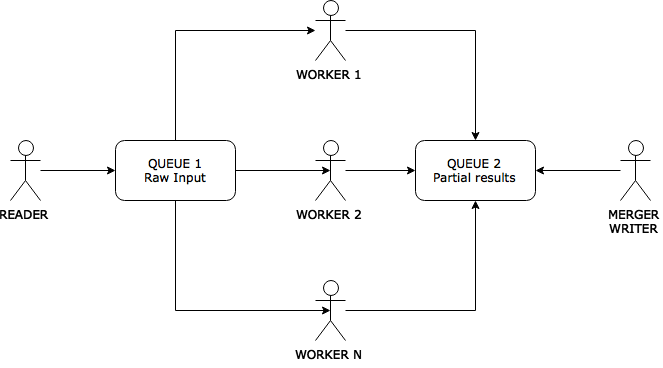
\includegraphics[width=\textwidth]{Figures/computeFrequencies.png}
\caption{Schema logico di computeFrequencies.py}
\end{figure}
\item Il codice del progetto è stato migrato alla versione 3.4 di Python che include un'interessante funzionalità: i dizionari a chiave condivisa\footnote{\url{https://www.python.org/dev/peps/pep-0412/}}. Questa caratteristica consente all'interprete Python di allocare memoria una sola volta per memorizzare le chiavi dei dizionari tra più istanze della stessa classe. Poiché lo script prevede una classe per rappresentare un processo e \texttt{Counter}, la classe utilizzata per contare le frequenze, è derivata dalla classe dizionario, questa modifica porta un significativo miglioramento del consumo di RAM dello script. Da alcuni test di verifica, il risparmio di memoria si è mostrato superiore al 50\%.
\item Nonostante la miglioria precedente, per il calcolo di tutte le frequenze dei bigrammi lo script richiede un quantitativo di RAM superiore a quello disponibile nella macchina di sviluppo. Si è quindi scelto di eseguirlo su una macchina virtuale Amazon EC2 di tipo \texttt{c3.2xlarge} con 8 CPU virtuali e $\SI{15}{\gibi\byte}$ di RAM. Il programma ha quindi svolto il suo compito in 1018 secondi (circa 17 minuti), con un picco di occupazione RAM intorno ai $\SI{13}{\gibi\byte}$.
\end{itemize}

\section{Scelta del DBMS}
\label{dbms}
Le occorrenze calcolate sono memorizzate in file con la seguente sintassi:

\indent{\texttt{Ngramma Frequenza}}

Le frequenze sono quindi da memorizzare in una base di dati che conservi queste coppie (chiave, valore) e ne consenta l'interrogazione in modo estremamente efficiente. Per stabilire infatti la migliore correzione possibile per una parola, come abbiamo visto nel capitolo \ref{cap_teoria}, è necessario calcolare un grande numero di probabilità. Per questo il DBMS Redis\footnote{\url{http://redis.io/}} fa al caso nostro \cite{nltkredis}. Redis è un database NoSQL ultra efficiente per memorizzare nella RAM coppie chiave-valore, che possono facoltativamente essere salvate su disco per garantire la persistenza. 

Le prestazioni di Redis variano, come è ovvio, dalla potenza dell'host su cui il server è installato ma anche dalla tipologia di connessione tra client e server (via TCP oppure UNIX socket). In linea di massima è comunque possibile affermare che Redis è in grado di servire oltre 100\,000 query/s.

Poiché per sua natura Redis mantiene tutte le informazioni direttamente in memoria è imporante che il server sia dimensionato correttamente in termini di RAM. In particolare, per questa installazione che contiene tutti gli unigrammi e i bigrammi il processo \texttt{redis-server} occupa (a caricamento completato) circa $\SI{1,7}{\gibi\byte}$.
La soluzione scelta per la produzione è su una VPS dedicata allo scopo con $\SI{2}{\gibi\byte}$ di RAM, disco SSD e connettività a $\SI{1}{GBps}$.

	\begin{mdframed}[style=indepth]
		\begingroup
		\setlength{\fboxsep}{0pt}%  
		\colorbox{black!50!white}{\makebox[\linewidth]{\textcolor{white}{\parbox[c][.8cm][c]{\linewidth}{\centering\textsc{A look into the world of NoSQL databases}}}}}
		\endgroup
		\hrule\vspace*{2mm}
		\hspace{.03\linewidth}\begin{minipage}{.94\linewidth}
NoSQL databases provide a mechanism for storing and retrieving data that is memorized in a different way than the tabular relations used in relational DBs. 

NoSQL databases are designed in contrast to relational databases, which were first introduced by Codd, an English computer scientist. He used the definition of a mathematical relation to organize data into one or more tables of rows and columns.

NoSQL databases feature highly optimized key-value operations (i.e., storing and reading a value given a key). Datastore of this kind may not require fixed table schemas and usually avoid join operations.

The term gained popularity in early 2009 with the advent of big data. In fact NoSQL DBs are often employed in real-time web applications and those requiring fast computation of a huge amount of data.
The benefits include:
\begin{itemize}
\item Scalability and superior performances;
\item Capability to memorize large volumes of structured and unstructured data;
\item An efficient architecture that can easily scale out;
\item Most implementations are open source.
\end{itemize}
Instead, the downsides are:
\begin{itemize}
\item Immaturity;
\item No support for a well-known and standardized language, as SQL;
\item No ACID transactions;
\item Many data structures (objects) cannot be easily represented as key-value pairs without a complex serialization.
\end{itemize}
		\end{minipage}
	\end{mdframed}


\section{Aggiornamenti in tempo reale}
Per fare in modo che il sistema proposto migliori con il tempo proponiamo una soluzione che migliori costantemente la base di dati su cui lavora l'algoritmo. Come già spiegato, tutto il lavoro di correzione si basa sulle probabilità ottenute dall'elaborazione di Wikipeida. La sorgente di dati non è stata scelta a caso: Wikipedia è continuamente aggiornata dagli utenti che correggono (inevitabili) errori e aggiungono contenuti.
Aggiornando quindi il nostro database i dati in esso contenuti vengono continuamente raffinati e, speranzosamente, offriranno una qualità della correzione sempre migliore.

\subsection{MediaWiki API}
\label{wikiapi}
Wikipedia, oltre al servizio di dump descritto nel paragrafo \ref{dump}, offre anche un insieme di API che consente a bot e terze parti di recuperare ed eventualmente modificare i dati. Il servizio di API, per la versione italiana, è disponibile presso \url{http://it.wikipedia.org/w/api.php}. Esistono diversi wrapper per l'API, ma spesso sono incompleti e poco aggiornati rispetto alle ultime versioni dell'interfaccia. Pertanto è stata creata una nuova classe Python che astrae l'interfaccia offrendo due metodi:
\begin{itemize}
\item \texttt{getRecentChanges}: restituisce una lista di (al più 500) oggetti JSON dove ciascuno rappresenta una modifica a una pagina di Wikipedia. È possibile specificare anche la data e l'ora da cui partire a recuperare le modifiche.
\item \texttt{getPageReviews}: a partire da una lista di identificativi di revisione, recupera il testo di ciascuna delle pagine a cui le revisioni fanno riferimento prima e dopo di esse.
\end{itemize}
La classe è disponibile nel repository del progetto.

\chapter{Implementazione del sistema}

\section{Schema architetturale completo}
Come si è potuto evincere dal capitolo precedente, il sistema è composto da diverse parti. Ciascuna di esse interagisce con le altre in un modo ben definito. Chiariamo meglio l'architettura completa con uno schema, spiegato nel dettaglio di seguito.
\begin{figure}[h]
\centering
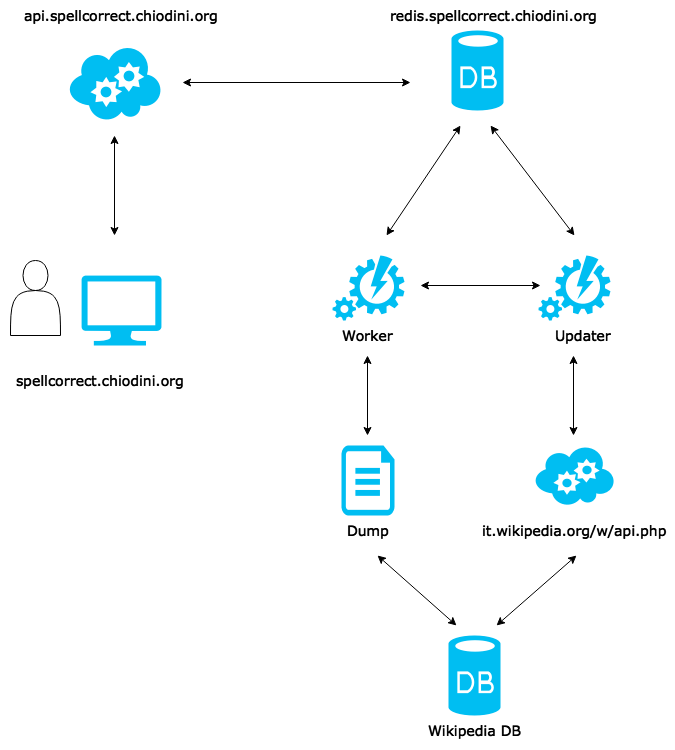
\includegraphics[width=\textwidth]{Figures/architecture.png}
\caption{Architettura del sistema}
\end{figure}

\begin{itemize}
	\item 
\url{spellcorrect.chiodini.org} è servito da Google App Engine\footnote{\url{https://cloud.google.com/appengine/}} ed è costituito da una pagina statica (e alcuni asset). Essa contiene un'area dove l'utente inserisce la parola o la frase da correggere; questa verrà inviata al servizio di API tramite richiesta AJAX.
	\item 
\url{api.spellcorrect.chiodini.org} è una web API, servita sempre da Google App Engine. Essa è tecnicamente realizzata tramite Flask\footnote{\url{http://flask.pocoo.org/}}, un microframework che consente di realizzare un web server usando come linguaggio Python.

La definizione dell'API è semplice: è necessario fare una richiesta a

\makebox[\linewidth]{\texttt{http://api.spellcorrect.chiodini.org/correct/<str>}}
sostituendo \texttt{<str>} con la parola o la frase da correggere. Il servizio risponde nella notazione JSON. Ecco un esempio tipico di risposta:
\begin{lstlisting}[language=json, numbers=none]
{
 "cache": false,
 "corrected": "eccezione", 
 "elapsed_time": "0:00:01.719220",
 "queries": 36,
 "input": "eccezzione"
}
\end{lstlisting}
I campi della risposta hanno i seguenti significati:
\begin{itemize}
\item \texttt{input} contiene l'input ricevuto;
\item \texttt{corrected} contiene la miglior correzione che il sistema è riuscito a calcolare per quell'input;
\item \texttt{elapsed\_time} indica il tempo, con precisione in microsecondi, impiegato per l'elaborazione;
\item \texttt{queries} indica il numero di query effettuate al database Redis;
\item \texttt{cache} indica se la risposta è stata calcolata al momento oppure recuperata dalla cache (cfr. \ref{cache}).
\end{itemize}

\item
\url{redis.spellcorrect.chiodini.org} ospita il DBMS Redis che si mette in ascolto sulla porta \texttt{TCP/6379}. Il DBMS è stato installato su una VPS (cfr. \ref{dbms}). 

\item
La restante parte dello schema rappresenta quanto già ampiamente discusso nel capitolo precedente. Le frequenze iniziali vengono memorizzate in Redis dopo essere state ottenute elaborando il dump. Gli aggiornamenti continui sono invece realizzati tramite un modulo (``Updater'' nello schema in figura) che periodicamente interroga le API di Wikipedia e processa le eventuali modifiche delle frequenze inviandole sempre a Redis.
\end{itemize}

\section{Algoritmo}
L'algoritmo di base è tratto da un articolo di Peter Norvig \cite{norvig}, che è l'attuale direttore del dipartimento di Ricerca presso Google. Rispetto alla versione originale sono stati modificati diversi punti, in accordo alla teoria definita nel capitolo \ref{cap_teoria}.

Lo schema riporta i passi essenziali dell'algoritmo di correzione:
\begin{itemize}
\item L'input viene ricevuto dall'applicazione Flask.
\item Per ciascuna parola presente nell'input, si procede alla generazione di tutte le parole candidate a sostituire quella presente. Per fare ciò, all'avvio viene precaricato in memoria tutto il dizionario delle parole conosciute. Tutte le parole presenti nel dizionario, aventi una distanza di  Damerau–Levenshtein (cfr. \ref{distanzadameraulev}) inferiore o uguale a due rispetto all'input, vengono considerate possibili candidati.
\item Per ogni candidato vengono effettuate tre query al database che misurano la probabilità del candidato di per sè e quella rispetto alla parola precedente e seguente (naturalmente ove applicabile). Viene inoltre considerata anche la probabilità basata sulla distanza Damerau–Levenshtein a cui la parola si trova rispetto a quella originale. Per un approccio rigoroso, si riveda il paragrafo \ref{probabilita}.
\item Il candidato con la probabilità più alta viene considerato il migliore e restituito come soluzione. È importante notare che anche la parola stessa originaria costituisce un candidato: essa infatti potrebbe essere corretta e non necessitare di alcuna alterazione.
\end{itemize}
\begin{figure}[h]
\centering
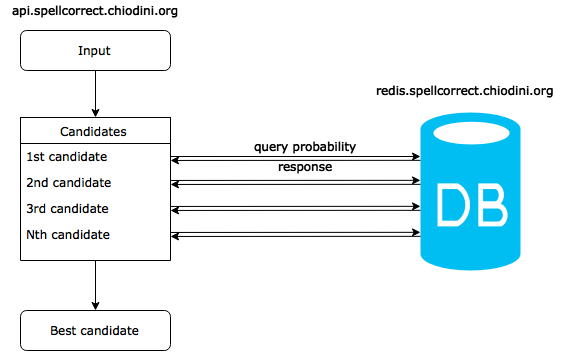
\includegraphics[width=\textwidth]{Figures/original_algorithm.png}
\caption{Algoritmo in dettaglio}
\label{fig:algoritmo}
\end{figure}

\pagebreak

\section{Efficienza}
I paragrafi seguenti spiegano i principali accorgimenti che sono stati adottati per rendere il sistema il più efficiente possibile.

\subsection{Ottimizzazione dell'algoritmo}
A un lettore attento non sarà sfuggito che l'algoritmo mostrato in figura \ref{fig:algoritmo} esegue un gran numero di interrogazioni sul database. Poiché client e server sono due host distinti, ogni query avrà un tempo di esecuzione pari alla latenza tra i due host sommata al tempo di esecuzione dell'interrogazione stessa. 

Redis è in grado di rispondere a una query in un tempo quasi sempre inferiore al millisecondo, ma la latenza tra due host su una rete geografica può essere anche 100 volte tanto. Essendo molto alto il numero delle interrogazioni è necessario evitare che per ciascuna sia necessario lo scambio di pacchetti TCP andata e ritorno: ciò porta a tempi di risposta complessivi inaccettabili.

Per risolvere il problema e ridurre drasticamente il tempo complessivo di risposta sfruttiamo una funzionalità di Redis, ``pipeline'', che consente di bufferizzare le query ed eseguirle tutte in un'unica volta.

Supponiamo che per correggere una certa frase servano 5000 query, che la latenza tra i due host sia di 50 ms e che Redis risponda a tutte le query in 1 ms: la tabella mostra un confronto tra i tempi dei due algoritmi.
\begin{table}[h]
\centering
\begin{tabular}{lrrl}
\toprule
Metodo		&	Latenza TCP					&	Tempo query		&	Tempo globale	\\
\midrule
Originale	&	$5000 \cdot 2 \cdot 50$ ms& $5000 \cdot 1$ ms	&	$\sim$ 8 min		\\
Ottimizzato	&	$1 \cdot 2 \cdot 50$ ms		& $5000 \cdot 1$ ms	&	$\sim$ 5 sec		\\
\bottomrule
\end{tabular}
\caption{Confronto tra i tempi di risposta dei due algoritmi}
\end{table}

\begin{figure}[h]
\centering
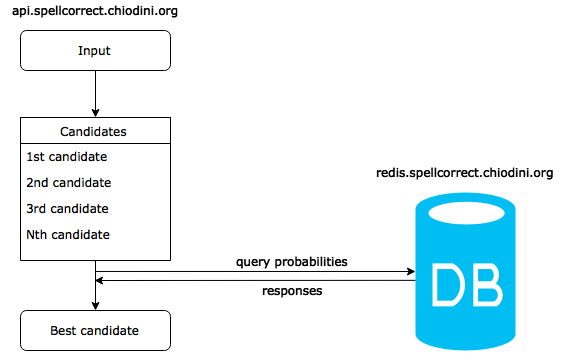
\includegraphics[width=\textwidth]{Figures/improved_algorithm.png}
\caption{Algoritmo ottimizzato}
\end{figure}
\subsection{Cache}
\label{cache}
Poiché più persone potrebbero richiedere la correzione delle stesse parole nel giro di poco tempo, ha senso mantenere una cache dei risultati. Questo permette di evitare il ricalcolo delle probabilità, che risulta essere molto oneroso.

All'interno della piattaforma App Engine è possibile sfruttare Memcached\footnote{\url{http://memcached.org/}}, un sistema distribuito ad alte prestazioni per salvare in memoria oggetti. Per quanto il progetto Memcached nasca e resti generico, esso è frequentemente impiegato come meccanismo di cache per alleviare il carico del database e velocizzare applicazioni web dinamiche e servizi di API.

Il funzionamento è tanto potente quanto semplice. Memcached prevede una chiave (in questo caso l'input), un valore (salviamo l'intero oggetto della risposta) e una scadenza. Ad ogni chiamata all'API viene eseguito questo codice (riportato nella sua versione essenziale):
\begin{lstlisting}[language=Python, numbers=none]
# Try to save resources and reduce response time retrieving
# the answer from the cache.
res = memcache.get(words_str)

# If the response has not been found in the cache:
if res is None:

    # Compute it.
    res = self.parse(words_str)
    
    # Add it to the cache (expire time 1 day).
    memcache.add(words_str, res, 86400)
\end{lstlisting}
\subsection{Scalabilità}
Oltre alle misure descritte nei due paragrafi precedenti si è ritenuto opportuno tenere in considerazione particolare la scalabilità del servizio di API. La piattaforma di produzione scelta, Google App Engine, consente infatti di lavorare sul concetto di istanza per garantire alta affidabilità ed elevate prestazioni.

Il meccanismo è semplice: la piattaforma monitora continuamente svariati parametri sulle risposte fornite dall'applicazione, di cui il più importante è il tempo medio di risposta. Quando quest'ultimo valore aumenta oltre una soglia ritenuta inaccettabile è evidente che un'instanza dell'applicazione non è sufficiente a soddisfare il carico corrente sul server e ne viene pertanto lanciata un'altra. In modo analogo, quando l'utilizzo medio delle risorse di un'instanza (CPU, RAM) diventa irrisorio App Engine decide di terminare l'istanza riducendo il costo complessivo.

Tutti i parametri di configurazione relativi alle istanze sono manipolabili nel file \texttt{app.yaml} e includono, oltre a quanto già visto, la scelta delle caratteristiche hardware virtuali dell'istanza e la possibilità di averne un certo numero sempre attive, pronte a rispondere alle richieste.
\chapter{Risultati}
Valutare quanto un correttore ortografico automatico sia buono non è facile. La maggior parte della letteratura su questo tema esegue dei test partendo da un elenco noto di errori ortografici e della loro esatta correzione, valutando quindi la percentuale di casi in cui il sistema ha dato l'esito atteso.

È però quasi impossibile fare una simile operazione con il nostro correttore in lingua italiana, banalmente perché non esiste un insieme di dati di questo tipo disponibile. Sarebbe possibile crearlo da zero, ma si rischierebbe un forte effetto di bias\footnote{\url{http://it.wikipedia.org/wiki/Bias_induttivo}}: i dati rischierebbero di essere costruiti appositamente per questo algoritmo di correzione. Di fatto verrebbe quindi valutata una correttezza specifica ma molto poco generica, rendendo così il risultato privo di interesse statistico.

\section{Si può fare di meglio?}
Alcuni aspetti del progetto possono essere estesi e migliorati:
\begin{itemize}
\item Tutti i programmi per l'elaborazione del codice supportano completamente la codifica UTF-8 dello standard Unicode, tuttavia lo stesso non si può dire per l'algoritmo di correzione in sè. Esso infatti, per ridurre il numero possibile di candidati alla correzione, considera solo caratteri minuscoli dell'alfabeto latino. Almeno il supporto alle lettere maiuscole e alle lettere accentate dovrebbe essere offerto. Dustin Boswell, in una sua ricerca del 2004 \cite{GeneratingCandidates}, esplora alcune strutture dati avanzate che sembrano essere promettenti per questo impiego.

\item L'algoritmo per la divisione del testo in parole utilizzato è banale: il carattere spazio ha la funzione di separatore. Questo non è evidentemente sempre vero anche considerando solo la lingua italiana: due parole potrebbero essere separate anche da un apostrofo. Questo problema è noto in letteratura come ``Word segmentation'' ed è un incubo se si considera, ad esempio, la lingua cinese dove alcune nostre frasi sono rappresentate con sequenze di una manciata di caratteri senza spazio. 

La divisione in parole resta comunque un problema anche considerando solo la lingua italiana: si prendano come esempio i due spezzoni di frase ``insufficienti modi'' e ``in sufficienti modi''. Un errore ortografico potrebbe essere anche il mancato inserimento dello spazio (o viceversa la sua aggiunta involontaria). Già questo piccolo esempio mostra come la divisione in parole sia a sua volta un sottoproblema estremamente vasto e risolto, ancora una volta, in modo statistico.

\item In un mondo globalizzato è oggi difficile pensare di realizzare un programma che funzioni solo in una sua piccola parte. Eppure per alcuni compiti piuttosto specifici è ancora necessario ragionare per area geografica. Uno di questi è sicuramente quello della correzione ortografica, il che lascia spesso delusi gli utenti, desiderosi di una soluzione universale. I risultati più promettenti in questo campo sembrano arrivare dai laboratori IBM \cite{languageindependent}.

\end{itemize}

\section{Pubblicazione del lavoro}
\label{pubb}
L'intera piattaforma di correzione, che comprende tutti i programmi Python che compongono i vari passaggi, è stata pubblicata su un repository di GitHub nel profilo dell'autore\footnote{\url{https://github.com/lucach/spellcorrect}} sotto licenza AGPL. L'impiego del sistema di controllo versione Git sin dalle prime fasi della programmazione ha consentito uno sviluppo particolarmente efficace, grazie alle funzionalità di branch e di revert delle ultime modifiche.

Gli indirizzi di riferimento a cui trovare l'applicazione sono:

\begin{itemize}
\item Sito web per utenti finali: \url{http://spellcorrect.chiodini.org}
\item API: \url{http://api.spellcorrect.chiodini.org}
\end{itemize}

%\include{Chapters/Chapter04} % Chapter 4 - empty template

%----------------------------------------------------------------------------------------
%	THESIS CONTENT - APPENDICES
%----------------------------------------------------------------------------------------

%\appendix

%\part{Appendix} % New part of the thesis for the appendix

%\include{Chapters/Chapter0A} % Appendix A
%\include{Chapters/Chapter0B} % Appendix B - empty template

%----------------------------------------------------------------------------------------
%	POST-CONTENT THESIS PAGES
%----------------------------------------------------------------------------------------

\cleardoublepage% Bibliography

\label{app:bibliography} % Reference the bibliography elsewhere with \autoref{app:bibliography}

\manualmark
\markboth{\spacedlowsmallcaps{\bibname}}{\spacedlowsmallcaps{\bibname}} 
\refstepcounter{dummy}

\addtocontents{toc}{\protect\vspace{\beforebibskip}} % Place the bibliography slightly below the rest of the document content in the table of contents
\addcontentsline{toc}{chapter}{\tocEntry{\bibname}}

\bibliographystyle{plainnat}

\bibliography{Bibliography} % Bibliography

%\cleardoublepage% Colophon (a brief description of publication or production notes relevant to the edition)

\pagestyle{empty}

\hfill

\vfill

\pdfbookmark[0]{Colophon}{colophon}

\section*{Colophon}

This document was typeset using the typographical look-and-feel \texttt{classicthesis} developed by Andr\'e Miede. The style was inspired by Robert Bringhurst's seminal book on typography ``\emph{The Elements of Typographic Style}''. \texttt{classicthesis} is available for both \LaTeX\ and \mLyX: 

\begin{center}
\url{http://code.google.com/p/classicthesis/}
\end{center}

\noindent Happy users of \texttt{classicthesis} usually send a real postcard to the author, a collection of postcards received so far is featured here: 

\begin{center}
\url{http://postcards.miede.de/}
\end{center}
 
\bigskip

\noindent\finalVersionString % Colophon

%\cleardoublepage% Declaration

\refstepcounter{dummy}
\pdfbookmark[0]{Declaration}{declaration} % Bookmark name visible in a PDF viewer

\chapter*{Declaration} % Declaration section text

\thispagestyle{empty}

Put your declaration here.
\bigskip
 
\noindent\textit{\myLocation, \myTime}

\smallskip

\begin{flushright}
\begin{tabular}{m{5cm}}
\\ \hline
\centering\myName, \today \\
\end{tabular}
\end{flushright}
 % Declaration

%----------------------------------------------------------------------------------------

\end{document}
